\subsection{The Ames Assay}
The Ames test is a widely-used \textit{in vitro} mutagenicity assay essential to drug development. Ames data is explicitly required by many regulatory guidelines, such as \gls{ich} guideline S2 (R1) \cite{ich_ich_2013}. It thus represents a high bar to market access for pharmaceuticals, with many compounds rejected early in the case of an Ames-positive outcome \cite{honma_improvement_2019}.

In the Ames assay, a histidine-deficient substrate is inoculated with strain of auxotrophic mutant histidine-dependent Salmonella typhimirium \cite{ames_improved_1973}. This dependence is introduced via a mutation at the histidine operon \cite{ames_improved_1973}. A suspected mutagenic compound is then introduced. If the mutagen-containing substrate shows significantly greater colony growth than a control, the test-molecule has reversed the histidine-dependence mutation and is mutagenic. This simplicity has resulted in the Ames test having an excellent inter-laboratory replicability of 85\% \cite{kamber_comparison_2009}.

Different \textit{S. typhimurium} strains detect various mutagenicity mechanisms, which can be categorized into substitution mutations (SNPs) or frameshift mutations \cite{lui_mechanistic_2023}. The Ames test also includes S9 rodent liver homogenate, enabling the detection of mutagens that require metabolic activation \cite{maron_revised_1983, ames_improved_1973}.

\subsection{QSAR Modelling}
As the Ames test costs approximately \$2000 per chemical and the CAS reigstry grows by over 4000 molecules daily, the cost of \textit{in vitro} screening for every new chemical quickly becomes prohibitive \cite{honma_improvement_2019}.

To address this problem, \textit{in silico} \gls{qsar} models have been developed to provide cheaper and higher-throughput methods of Ames screening \cite{furuhama_evaluation_2023}. The use of such models is recommended within \gls{ich} guideline M7 (R1) for the control of mutagenic impurities in pharmaceuticals and the European Union's \gls{reach} agreement \cite{european_communities_regulation_2006, ich_assessment_2017, honma_improvement_2019}. \Gls{aicis} and \gls{fda} have also provided guidelines for implementing \textit{in silico} toxicity evaluation methods \cite{aicis_guide_2022, han_fda_2023}.

\subsection{Current Models}
The input to many Ames \gls{qsar} models are \glspl{mf}. \gls{mf}, as seen in \cref{fig:ndma_fp}, are vectorised binary representations of a molecule’s chemical features \cite{capecchi_one_2020}. 

\begin{figure}[H]
    \centering
    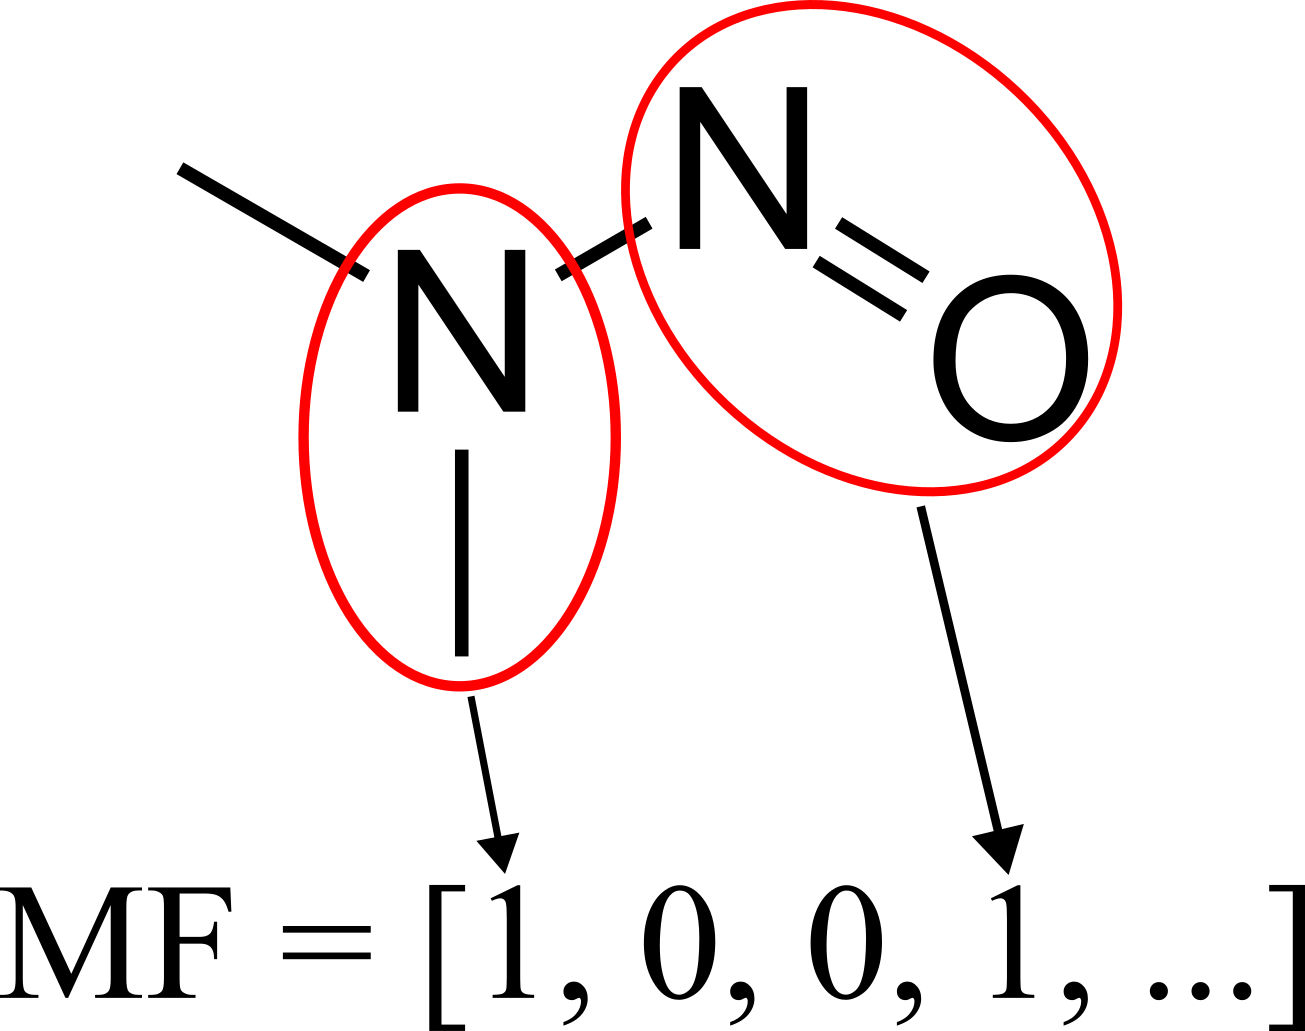
\includegraphics[width=0.35\linewidth]{Images/NDMA Fingerprint.png}
    \caption{An illustrative examples of the hashing of different \gls{ndma} substructrures into the \gls{mf} bit vector.}
    \label{fig:ndma_fp}
\end{figure}

Two fingerprinting methodologies are commonly applied to molecules within the Lipinski Limits. 
Structural key \glspl{mf}, such as \gls{maccs} keys seen in \cref{fig:maccs}, encode the presence of a set of predefined chemical substructures into a binary vector \cite{durant_reoptimization_2002, seo_development_2020}.
Hash \gls{mf} \textit{de novo} numerically encode non-predefined substructures. The archetypal \gls{morgan} \gls{mf} shown in \cref{fig:morgan} hashes the local environment (of arbitrary size) around each atom and encodes this into the bit vector representation \cite{rogers_extended-connectivity_2010}.

\begin{figure}[H]
    \centering
    \begin{subfigure}[t]{0.48\textwidth}
        \centering
        \begin{align*}
            \text{MACCS} &= \begin{bmatrix}
               x_{1} \\
               x_{2} \\
               \vdots \\
               x_{166}
             \end{bmatrix}
            \rightarrow \{0, 1\}^{166}
        \end{align*}
        \caption{\gls{maccs} fingerprint are bit vector encoding the presence (1) or absence (0) of a set of 166 predefined molecular substructures. The index of each substructure is unique.}
        \label{fig:maccs}
    \end{subfigure}
    \hfill
    \begin{subfigure}[t]{0.48\textwidth}
        \centering
        \begin{align*}
            \text{ECFP} &= \begin{bmatrix}
               x_{1} \\
               x_{2} \\
               \vdots \\
               x_{n}
             \end{bmatrix}
            \rightarrow \{0, 1\}^n
        \end{align*}
        \caption{Morgan fingerprints encode an arbitrarily sized set of non-predefined molecular substructures into a bit vector of arbitrary length.}
        \label{fig:morgan}
    \end{subfigure}
    \caption{Different molecular fingerprinting techniques and their dimensionalities.}
\end{figure}

\textbf{Number} of the 22? Ames models presented in the Second Ames International Challenge by \textcite{furuhama_evaluation_2023} utilise \gls{mf}-type input data.



Structural Key
